\chapter{Разработка собственного решения с использованием белорусской криптографии}

	\section{Поиск существующих имплементаций}
	
	Первой задачей практической части было нахождение существующих реализаций подробно описанных
	выше протоколов с целью дальнейшей работы над криптографическим аспектом этих реализаций.
	В качестве основного протокола для модификаций был выбран протокол ZigBee. Были поставлены
	следующие задачи:
	
	\begin{itemize}
		\item поиск имплементации протокола ZigBee, позволяющей вносить модификации; 
		\item поиск устройств (микроконтроллеров), способных работать на этой имплементации;
		\item изменение или полная замена криптографической составляющей в имплементации.
	\end{itemize}

	К сожалению, открытых реализация оказалось немного. Практически не было найдено библиотек,
	реализующих в полной мере последнюю версию протокола. Проблема заключается в том, что сама
	спецификация находится в закрытом доступе. Для получения спецификации необходимо стать
	членом ZigBee Alliance, что осуществляется на платной основе. Аналогично, все имплементации
	протокола ведущими технологическими компания также являются закрытыми. Это связано с
	коммерческой составляющей, поскольку компании получают прибыль, реализуя устройства
	на собственных прошивках.
	
	По совокупности вышеописанных факторов был выбран другой подход, который не привязан
	к определённому протоколу. Суть данного подхода заключается в самостоятельной реализации
	криптографического уровня защиты и применении его поверх установленного соединения между
	управляющим устройством (хабом) и конечным устройством. В качестве конечного устройства
	в данной работе был выбран прототип умной лампочки.
	
	
	\section{Выбор компонентов и технологий для реализации}
	
	Обновлённые практические задачи были сформулированы следующим образом:
	
	\begin{itemize}
		\item выбор микроконтроллера, который будет служить прототипом умного устройства,
		с возможностью его программирования и прошивки;
		\item установка соединения между управляющим и умным устройствами. Для простоты в качестве
		управляющего устройства в данной работе используется компьютер;
		\item разработка кода (прошивки) для умного устройства (контроллера), а также клиентского
		приложения для управляющего устройства;
		\item реализация защищённого обмена сообщениями с использование белорусского криптографического
		стандарта СТБ 34.101.77;
		\item модификация стандарта с изменением значения некоторых его параметров;
		\item оценка стойкости видоизменённого решения.
	\end{itemize}

	В качестве микроконтроллера был выбран ESP8266 (модель NodeMCU V3). Это недорогая модель от
	китайской компании Espressif Systems. Её большим преимуществом является встроенный Wi-Fi модуль. 
	Помимо поддерживаемых протоколов Wi-Fi 802.11 b/g/n и режимов работы как в качестве точки доступа,
	так и клиента, микроконтроллер отличается встроенным стеком TCP/IP.
	
	Для программирования данной модели существует широкий выбор языков, платформ и сред, среди
	которых Arduino IDE, Espressif IoT Development Framework (официальный фреймворк от разработчика)
	и многие другие. В данной работе была выбран инструмент PlatformIO \cite{platformio}. Это
	кроссплатформенная интегрированная среда разработки, построенная на основе редактора Microsoft 
	Visual Studio Code, а также встроенный отладчик, статический анализатор кода и система сборки.
	Платформа поддерживает большое количество микроконтроллеров, среди которых в том числе есть
	ESP8266 NodeMCU. На сайте также представлен широкий выбор библиотек и примеров с кодом.
	Языком разработки на платформе является C++.
	
	При выборе инструментов и технологий для разработки также рассматривались варианты использования
	более высокоуровневых языков программировая, таких как Java \cite{microej} или .NET \cite{nanoFramework}.
	Однако наличие примеров, библиотек и большого сообщества разработчиков стало определяющим
	фактором при выборе PlatformIO. При этом для клиентского веб-приложения на управляющем устройстве
	(компьютере) была выбран язык программирования Java.
	
	
	\section{Работа с микроконтроллером ESP8266}
	
	\begin{figure}[h]
		\centering
		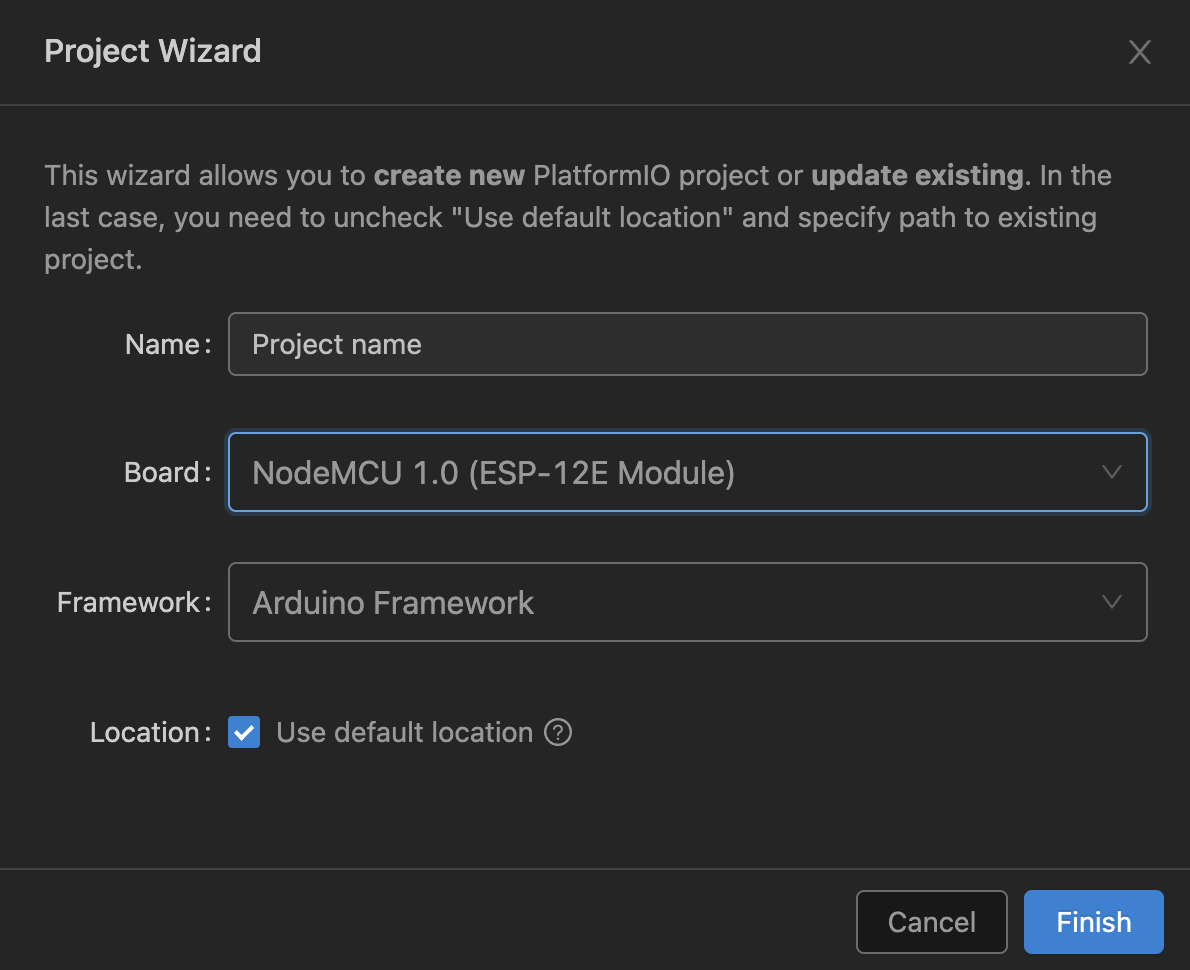
\includegraphics[scale=0.6]{resources/platformio-new-project}
		\caption{Меню создания нового проекта в PlatformIO}
		\label{fig4.1}
	\end{figure}
	
	Первым шагом при программировании микроконтроллера стало создание проекта при помощи PlatformIO.
	На этапе создания нового проекта появляется возможность выбора контроллера. Основными составляющими
	в проекте являются конфигурационный файл platformio.ini, в котором указывается модель контроллера,
	а также подключаемые к проекту библиотеки, и директива src, в которой должен содержаться код проекта.
	
	При первоначально настройке в папке src содержится единственный файл main.cpp. Он включает два
	метода. Метод setup() отвечает за первоначальную конфигурацию контроллера, а метод loop()
	повторяется всё время, пока контроллер подключен к питанию.
	
	Для знакомства с программированием данного типа контроллеров и изучения программных методов
	было реализовано несколько базовых примеров. Первым из них было мигание встроенного на контроллере
	индикатора. Затем были построены простейшие схемы с использованием макетной платы, диода и
	нескольких проводов. Мигание встроенного индикатора было заменено миганием диода. После этого
	был реализован пример управления диода по нажатию кнопки. Наконец, был задействован Wi-Fi модуль
	для управления диодом с компьютера. Данный пример был взят за основу практического прототипа. Более
	подробно работа прототипа и все этапа обмена сообщениями будут рассмотрены позже. Но перед этим
	перейдём к криптографической части данной работы.
	
	\begin{figure}[h]
		\centering
		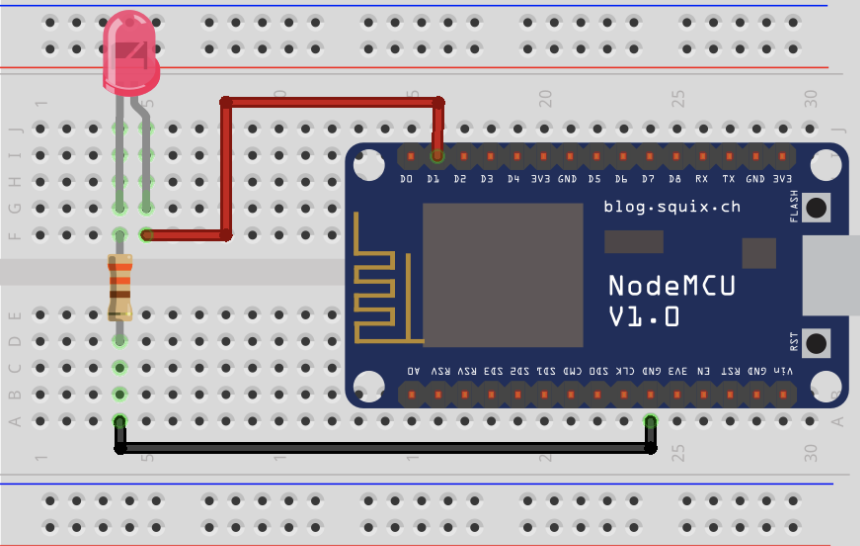
\includegraphics[scale=0.6]{resources/esp8266-control-led}
		\caption{Схема подключения диода к микроконтроллеру}
		\label{fig4.2}
	\end{figure}
	
	
	\section{Реализация и использование криптографического стандарта СТБ 34.101.77}
	
	\section{Модель прототипа}
	